\chapter{Methodology}\label{ch:methodology}

Following is a short overview of methodologies applied during crucial steps in our process that will be discussed in more detail in the following sections:

\begin{enumerate}
    \item Preparation
    \begin{itemize}
        \item Selecting a \gls{Blockchain} network
        \item Selecting the technology stack
    \end{itemize}
    \item Development
    \begin{itemize}
        \item Versioning
        \item Agile development
        \item End-to-end tests
    \end{itemize}
    \item Evaluation
    \begin{itemize}
        \item Test analysis
        \item Technical analysis
        \item Cryptocurrency transaction analysis
    \end{itemize}
\end{enumerate}

\section{Preparation}\label{sec:preparation}

\subsection{Selecting a blockchain network}\label{subsec:selection-of-blockchain-network2}

To select the most feasible blockchain network, we compared the findings in \cref{sec:voting-systems} with those in \cref{subsec:comparison-of-turing-complete-blockchains}.

\subsection{Selecting the technology stack}\label{subsec:selection-of-technology-stack}

Similarly, after researching possible development tools (see \cref{sec:development-tools}), we considered a suitable technology stack.

\begin{figure}[H]
    \begin{subfigure}[b]{\textwidth}
        \centering
        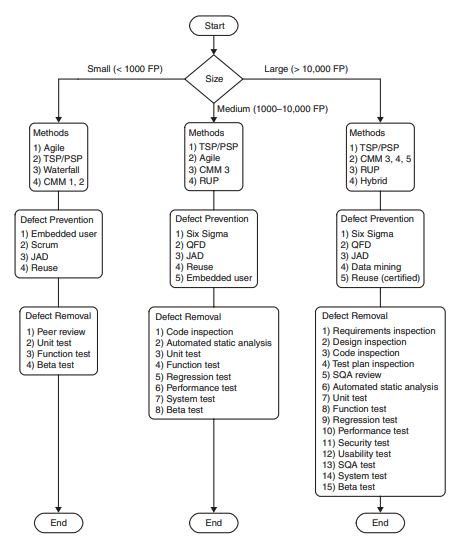
\includegraphics[width=0.7\textwidth]{jones-2010-development-methods}
        \caption[Success rates of development methods]{Success rates of development methods in relation to project size~\autocite[11]{jones_software_2010}}
        \label{fig:success-rates-development-methods}
    \end{subfigure}
    \begin{subfigure}[b]{\textwidth}
        \centering
        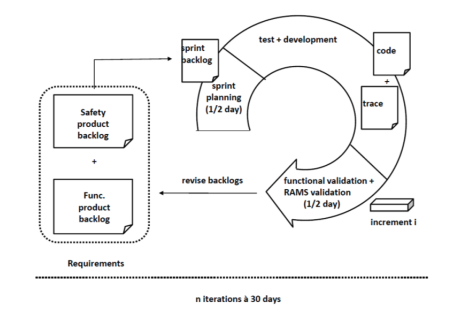
\includegraphics[scale=.8]{myklebust-2014-scrum}
        \caption[Scrum method]{Scrum method~\autocite[2]{myklebust_scrum_nodate}}
        \label{fig:scrum-method}
    \end{subfigure}
    \caption{Development methods}\label{fig:development-methods}
\end{figure}

\section{Development}\label{sec:development}

\subsection{Versioning}\label{subsec:versioning}

We used Git Workflows to version the project during development, which enabled parallel workflows depending on features and provided greater flexibility.
Furthermore, it enabled the analysis of code changes during our iterative process and revision of changes and is well-established in the software industry and does not have serious contenders that are also open-source.

\subsection{Agile development}\label{subsec:agile-development}

The development methods displayed in \cref{fig:success-rates-development-methods} are sorted according to their success rates.
As stated by~\textcite[10-12]{jones_software_2010}, projects with a size of less than 1000 function points are most likely to benefit from agile development methods.
The median size of function points is defined as 53 lines of JavaScript code by~\textcite{qsm_function_2009}.
Based on these findings, we applied agile development methods during the development process as the project's size was not anticipated to grow beyond the aforementioned dimensions.

However, we departed from the recommended defect prevention methods shown in~\cref{fig:success-rates-development-methods} since embedded user reviews mainly test the application’s frontend functionality.
Instead, the same goal could be achieved by applying Scrum methods and \gls{E2E} tests.

\subsection{Personal Scrum}\label{subsec:personal-scrum}

Despite this being a one-person project with different organizational requirements than projects developed by a team, we applied scrum methods (see \cref{fig:scrum-method}) during our development process.
As stated by \textcites{andrews_scrum_2017}{pahuja_scrum_2015}, this meant adapting scrum methods for personal use, enabling us to establish iterative processes to track the development process, evaluate intermediate results and remove defects (see~\cref{fig:scrum-method}).

\subsection{End-to-end tests}\label{subsec:end-to-end-tests}

Since peer reviews are no feasible option for defect removal in a single-person project, we employed E2E tests to check the application’s intended functionality and iteratively remove possible defects.
Also, in contrast to unit tests, \gls{E2E} tests provided the possibility to test entire workflows of the application, such as the registration or voting process.

\subsection{Atomic design}\label{subsec:atomic-design}


\section{Evaluation}\label{sec:evaluation}

The primary objective of this thesis was the development of a decentralized voting system under the assumption that such a system would dramatically improve upon fundamental properties of voting systems compared to analogous and centralized electronic systems.
For this, we first identified objectives based on a qualitative analysis of relevant research data (see~\cref{sec:voting-systems}) and quantified established \gls{E2E} election processes of analogous voting systems to convert them into software features mirroring the process.


\subsection{Tests}\label{subsec:tests}
\subsection{Cryptocurrency transaction analysis}\label{subsec:crypto-currency-transaction-analysis}